\chapter{Computational results} \label{ch:compresults}
%! Scopo degli esperimenti: analizzare la performance di ZI-Round nelle sue varie estensioni/varianti in termini di numero di soluzioni intere trovate e tempo di esecuzione.
The performance of the ZI-Round heuristic is analyzed in the following experiments, in which one extension at a time is changed from the default version. The main measures of interest are the number or percentage of integer solutions found, the quality of those solutions and the execution time of ZI-Round. \par 

First, in Section~\ref{sec:preliminary-exp}, two preliminary experiments are carried out: the first one concerning the comparison between the results obtained by default ZI-Round and those reported by C. Wallace  for the successful instances in \cite{wallace2010}; the second one concerning the comparison between the results obtained by default ZI-Round and those obtained by the \textit{zirounding} heuristic implemented in the non-commercial solver SCIP, on the same test-bed used by C. Wallace. These experiments serve as confirmation of the reliability of the ZI-Round implementation made by the author of this thesis. \par

In Section~\ref{sec:expsetup}, the experimental setup used for the set of experiments on the different versions of ZI-Round is presented. In particular, it comprises the specification of the hardware and software tools used, the description of the test-beds used for the experiments, the specification of the single measures performed on the instances and the aggregate measures computed on the test-beds. Also, a second interesting set of experiments that exploit the shift of dimensional space seen in the presolving process of CPLEX is introduced. \par 

In Section~\ref{sec:expresults} the experimental results on the test-beds described are presented and discussed, together with some example charts showing the behavior of the ZI-Round versions tested in terms of solution fractionality and solution cost, on two reference instances. The charts presented are made by the author of this thesis using the Gnuplot graphing utility \cite{gnuplot}, called directly from the main program through a pipe. The data portrayed by the charts is obtained from the experiments conducted.

\section{Preliminary experiments} \label{sec:preliminary-exp}

\subsection{Comparison with ZI-Round v2}
After implementing the default version of the ZI-Round heuristic, referred to as ZI-Round version $2$ (v$2$) in the original work by C. Wallace \cite{wallace2010}, a quick replicability experiment is carried out to check whether the custom implementation of the author of this thesis finds similar resulting objective values to those found by the implementation of C. Wallace, for the successful instances reported in the article. In particular, the test-bed contains $18$ instances taken from the MIPLIB $2003$ problem set \cite{miplib2003}, from which one instance is removed since it has ranged constraints that make it incompatible with the custom implementation. \par
The results of the replicability experiment are reported in Table~\ref{tb:exp-prelim-1}: the implemented default version of ZI-Round found a solution for $13$ of the $17$ instances for which ZI-Round v$2$ found a solution.
\begin{table}[]
	\centering
	\begin{tabular}{@{}lrrr@{}}
	\toprule
	Instance   & ZI-Round(implemented) & ZI-Round(v2) & zirounding(SCIP) \\ \midrule
	cap6000    & -2446875              & -2446875     & -2442801         \\
	fast0507   & 221                   & 200          & 288              \\
	fixnet6    & 12170                 & 4536         & 4482             \\
	manna81    & -11868                & -13164       & -13150           \\
	markshare1 & 230                   & 230          & 418              \\
	markshare2 & 167                   & 674          & 375              \\
	mkc        & Failed                & -346      & Failed           \\
	modglob    & 20786787           & 20786788     & 20757201      \\
	nsrand-ipx & 754880                & 69600        & Failed           \\
	pp08a      & 15000                 & 14300        & 13940            \\
	pp08aCUTS  & 16630           & 16630      & 15147      \\
	qiu        & 1805           & 1805      & 1805      \\
	set1ch     & 110242              & 107692     & 106027           \\
	seymour    & 454                   & 450          & 615              \\
	sp97ar     & Failed                & 1094926720   & Failed           \\
	timtab1    & Failed                & 1719551      & Failed           \\
	timtab2    & Failed                & 2449798      & Failed           \\ \bottomrule
	\end{tabular}
	\caption{Objective values obtained by different implementations of the default ZI-Round heuristic.}
	\label{tb:exp-prelim-1}
\end{table}

The failure of the custom implementation in $4$ instances is further analyzed in a second experiment, by comparing the results with those obtained by the \textit{zirounding} heuristic integrated in the non-commercial solver SCIP version $7$.$0$.$0$ \cite{scip}, which could not be extracted from the code of the version used in \cite{wallace2010}, leading to the implementation of ZI-Round v$2$. \par 

\subsection{Comparison with ZI-Round in SCIP}
To double check the reliability of the previous results, the test-bed is extended to the whole MIPLIB $2003$ problem set, which is the complete test-bed actually used by C. Wallace, from which the instances that are incompatible with ZI-Round are removed. The extended test-bed contains $59$ instances. The second preliminary experiment involves the comparison between default ZI-Round and \textit{zirounding}, to confirm the reliability of the implementation. \par 

The solver SCIP was downloaded with an academic license and set up to use only the \textit{zirounding} heuristic and stop the solving process at the root node of the decision tree. In particular, the following commands are issued:
\begin{enumerate}
	\item Disable all the heuristics: "\texttt{set heuristics emphasis off}"
	\item Enable the \textit{zirounding} heuristic: "\texttt{set heuristics zirounding freq 1}"
	\item Set the node limit to $1$: "\texttt{set limits nodes 1}"
	\item Disable all cut separators: "\texttt{set separating emphasis off}"
\end{enumerate}
Once SCIP is set up, the command to optimize a given problem is the following: "\texttt{read filename.mps optimize}". The execution and success of \textit{zirounding} can be verified by issuing the command "\texttt{disp stats}" after the problem optimization. \par

The complete results of the second experiment are omitted since almost all the additional instances not reported in Table~\ref{tb:exp-prelim-1} are unsuccessful for both the implementations being compared.  \par 

The results obtained by SCIP present the same $4$ failures mentioned previously. With some slight differences, which could be due to the newer versions of the solvers being used or performance variability factors, the custom implementation of ZI-Round made by the author of this thesis can be deemed as a reliable instance of the heuristic to be tested in the following experiments.

\section{Experimental setup} \label{sec:expsetup}

\subsection{Hardware and software tools}
%! Strumenti: specifiche PC, software/tools usati
All the experiments are performed on a Dell XPS $15$ $7590$, with an exa-core $4.5$ GHz i$7$-$9750$H processor and $16$ GB of RAM, using the Windows $10$ Pro version $2004$ operating system. \par

%! Software/tools usati
The solver used for obtaining the solutions of the continuous relaxations is CPLEX version $12$.$10$.$0$ with an academic license \cite{cplex}. Its interactive optimizer is also used for presolving problems and writing them to \texttt{mps} files.
The Dirent C API \cite{dirent} is used for easily scanning the instance files to read in the test folder.
The Gnuplot \cite{gnuplot} graphing utility is used to programmatically create the charts presented in this thesis using pipes to pass commands and data points to it directly from the main program.
The R language \cite{rlang} is used to easily manage the test results and compute the aggregate measures of interest.

\subsection{Test-bed collection}

%! Testbed: MIPLIBS + tipologie di istanze rimosse + numero istanze testate
The test-bed used for the experiments comprises the instances from the MIPLIB $2003$ \cite{miplib2003}, MIPLIB $2010$ \cite{miplib2010} and MIPLIB $2017$ \cite{miplib2017} problem collections, from which the instances that are incompatible with ZI-Round are removed.
The removed instances include: instances that are infeasible or unbounded; instances that have ranged constraints; instances that have semi-integer or semi-continuous variables according to the terminology used by CPLEX; and instances for which CPLEX is unable to solve the continuous relaxation or exceeds a set time limit of $300$ seconds. To simplify the detection of removable instances, a single run in which only the continuous relaxations are solved is performed on the union of the three problem collections: the function \texttt{CPXgetstat} of the CPLEX C API is used to get the solution status and the instances that do not have the status \texttt{CPX\_STAT\_OPTIMAL} are removed from the test-bed. After this pre-processing run, the test-bed obtained contains $1102$ instances.
To virtually increase the size of the test-bed and at the same time test the effect of the performance variability on the end results, the experiments are done using three random seeds. So the actual independent instances are instance-seed pairs, bringing the test-bed size to $3306$. \par 

%! Idea: vedere come cambia la performance lavorando nello spazio dei problemi presolved  creazione di un test-bed presolved usando l’interactive optimizer di CPLEX (breve descrizione), poi gli stessi test sono fatti su questo secondo test-bed
An interesting observation about the way in which CPLEX operates gives rise to an alternative test-bed that can easily be derived from the original one previously described.
When CPLEX solves the continuous relaxation of a problem instance, it applies a presolving process that skims through the problem at hand and reduces it to a different dimensional space in terms of number of variables and/or constraints, usually with a more compact matrix. However, after finding a solution for the modified problem, it converts it back to the original problem space and returns it. This behavior led the supervisor of this thesis D. Salvagnin to suggest performing a second set of experiments on the presolved version of the test-bed, exploiting the more compact formulations of the problems in the hope that ZI-Round could perform differently on the presolved test-bed. \par 

The interactive optimizer of CPLEX is used for the test-bed conversion: each instance file in \texttt{mps} format is read, the problem is presolved, written back in \texttt{pre} format, then read again and finally written back in \texttt{mps} format. This conversion process can be automated easily with a simple script, since the interactive optimizer of CPLEX is command line driven and accepts sequences of command strings in input. As done for the original one, the presolved test-bed undergoes the same pre-processing run that filters the instances by the continuous relaxation solution status, leading to the removal of $10$ more instances. So the presolved test-bed has a size of $1092$, which is increased to $3276$ by the use of the three random seeds. \par

%! modalità di test (test_folder), reporting dei risultati (file csv perché sono facilmente manipolabili)
The runs for the experiments on the test-bed folder rely on the Dirent C API to scan the instance files in a way that is easy to code. When each instance has been processed, its related measures are appended to a \texttt{csv} file that holds the test results. The choice of using \texttt{csv} files follows from the ease of processing that software tools as the R language provide for this file format.

\subsection{Performance measures and aggregate measures}

%! Misure riportate nei csv
The actual data reported in the test results files comprises: the name of the instance, the random seed used, the final solution cost, the final solution fractionality, the number of rounds performed by ZI-Round (outer loop iterations), the execution time taken by CPLEX to solve the continuous relaxation, the execution time of ZI-Round, the sum of the two times, and the gap of the solution found with respect to the optimal or best solution available for the given problem. \par 

%! Performance measures (misure aggregate) + come sono calcolate, specificando che sono state calcolate usando scripting in R
In order to evaluate the performance of ZI-Round on the test-beds, the following aggregate measures are computed by means of a script in the R language that processes the files of the test results and of the optimal or best objective values of the instances. \par
\subsubsection{Success rate}
The first aggregate measure is the success rate, which evaluates the number of integer solutions found by ZI-Round as a percentage. It is computed as the ratio between the number of instances whose solution has a zero fractionality and the total number of instances. \par
\subsubsection{Average gap}
The quality of the solutions found by ZI-Round is evaluated by the gap with respect to the optimal or the best solution available, which is computed as a percentage. When an optimal objective value is available, the gap is $0$\% if the optimal solution is found and $100$\% if the objective value is more than twice the optimal one. In case the optimal objective value is zero, the gap can only be either $0$\% for the optimal value or $100$\% for any other value found by ZI-Round. When an optimal objective value is not available but the best one found so far is, the gap is $0$\% if the value found by ZI-Round is less than or equal to it, and $100$\% otherwise. When no solutions have ever been found for the problem, thus no best objective value is available, the gap is $0$\% if any solution is even found and $100$\% otherwise. Programmatically, the script first computes the gap for each tested instance and adds the gap column to the test results file; then computes the average gap, which is the aggregate measure for the test-bed. \par
\subsubsection{Shifted geometric mean of execution times}
To evaluate the performance of ZI-Round in terms of execution time, two phases are taken into account: the phase in which CPLEX solves the continuous relaxation to produce the input initial solution for ZI-Round and the actual execution of the heuristic. Execution times are measured by means of calls to the functions \texttt{QueryPerformanceCounter} and \texttt{QueryPerformanceFrequency}, included in the \texttt{windows.h} header file, and are expressed in milliseconds. The aggregate measure involving execution times used to convey information about the performance of ZI-Round on the whole test-bed is the shifted geometric mean (SGM). 
For a sequence of measured execution times $\{t_i\}_{i=1}^{n}$ and a shift $s$, the SGM is given by:
\begin{equation}\label{eq:sgm}
	\sqrt[n]{\prod_{i=1}^{n}(t_i+s)} - s = e^{\dfrac{\sum_{i=1}^{n}\ln(t_i+s)}{n}}-s
\end{equation}
The second formulation of the SGM, i.e. the right member of Equation~\ref{eq:sgm} is useful for easily computing it in the R language as "\texttt{exp(mean(log(t + s))) - s}", where \texttt{t} is the vector of execution times and \texttt{s} is the chosen shift.
%! Perchè usare la media geometrica shiftata
The geometric mean is used in its shifted version to avoid giving the same relevancy, for example, to an improvement from $20$ to $10$ milliseconds and an improvement from $2000$ to $1000$ milliseconds.
The shifts used for the SGM of the continuous relaxation and ZI-Round execution times are of $1000$ and $10$ milliseconds, respectively. \par 
\subsubsection{Shifted geometric mean ratio of execution times}
A composite aggregate measure that is derived from the SGMs of the two execution times is the ratio between the SGM of the ZI-Round and continuous relaxation execution times, expressed as a percentage, which gives an idea of the fraction of time used by ZI-Round with respect to the time taken to solve the continuous relaxation of the problem.
\subsubsection{Shifted geometric mean of the number of rounds}
The shifted geometric mean is also used to compute the aggregate measure regarding the number of rounds, i.e. outer loop iterations, performed by ZI-Round. The shift used for this SGM is of $10$, since for most instances the number of rounds is less than $10$ but there are some outliers for which ZI-Round performs hundreds or thousands of rounds.

\section{Experimental results} \label{sec:expresults}

\subsection{Aggregate results on the test-beds}

%* COMMENTI TABELLE
The results of the experiments conducted are reported in Table~\ref{tb:results-normal} and Table~\ref{tb:results-presolved}, for the two test-beds, respectively. The ZI-Round version acronyms stand for, respectively: NSNF as in "No Shift Non-Fractional", i.e. no objective improvement; A0F as in "After 0 Fractionality", i.e. objective improvement after zero fractionality; WOBJ as in "Worst OBJ", i.e. worst-objective fractionality tie-breaks; SS as in "Sort Singletons"; Prop as in "Proposed". As for the acronyms of the aggregate measures, SR stands for "Success Rate" and SGM-R refers to the number of rounds, i.e. iterations of the outer loop of ZI-Round. \par
\begin{table}[ht]
	\centering
	\begin{tabular}{@{}lcccccc@{}}
	\toprule
	Version  & SR(\%) & SGM-LP(ms) & SGM-ZI(ms) & ZI/LP(\%) & Gap(\%) & SGM-R \\ \midrule
	Default  & 19.800 & 993.652    & 3.544      & 0.357     & 89.856  & 2.344 \\
	NSNF     & 19.830 & 1000.571   & 1.569      & 0.157     & 91.904  & 2.322 \\
	A0F      & 19.830 & 989.142    & 1.858      & 0.188     & 89.833  & 2.399 \\
	WOBJ     & 20.073 & 997.646    & 3.606      & 0.361     & 89.870  & 2.375 \\
	SS       & 19.800 & 998.354    & 3.595      & 0.360     & 89.856  & 2.344 \\
	Prop     & 20.103 & 998.812    & 2.039      & 0.204     & 89.664  & 2.573 \\ \bottomrule
	\end{tabular}
	\caption{Aggregate measures of the experimental results for the regular test-bed.}
	\label{tb:results-normal}
\end{table}
\begin{table}[ht]
	\centering
	\begin{tabular}{@{}lcccccc@{}}
	\toprule
	Version  & SR(\%) & SGM-LP(ms) & SGM-ZI(ms) & ZI/LP(\%) & Gap(\%) & SGM-R \\ \midrule
	Default  & 17.613 & 865.126    & 2.315      & 0.268     & 90.928  & 2.268 \\
	NSNF     & 17.613 & 867.309    & 0.926      & 0.107     & 92.844  & 2.210 \\
	A0F      & 17.613 & 868.319    & 1.125      & 0.130     & 90.919  & 2.285 \\
	WOBJ     & 17.705 & 864.727    & 2.352      & 0.272     & 91.084  & 2.310 \\
	SS       & 17.613 & 865.622    & 2.333      & 0.269     & 90.928  & 2.268 \\
	Prop     & 17.705 & 864.226    & 1.131      & 0.131     & 91.063  & 2.298 \\ \bottomrule
	\end{tabular}
	\caption{Aggregate measures of the experimental results for the presolved test-bed.}
	\label{tb:results-presolved}
\end{table}

%! Testbed normale vs presolved: sul testbed normale tutte le versioni ottengono success rate più alti e average gap più bassi rispetto a quanto ottenuto sul testbed presolved. --> Questa differenza supporta l'ipotesi che il presolving dei problemi porti ad vere formulazioni più compatte ma non necessariamente meno complesse da risolvere.
The results on the regular test-bed show that all the ZI-Round versions tested obtain higher success rates and lower average gaps with respect to the presolved test-bed. This difference of performance supports the hypothesis that the presolving process leads to problem formulations that are indeed more compact, but not necessarily less complex to solve. \par

%! SuccRate testbed normale: WOBJ è l'estensione che riesce a migliorare maggiormente il success rate, mentre NSNF e A0F danno solo dei piccoli miglioramenti. --> L'unione delle 3 estensioni A0F,WOBJ,SS nella versione PROPOSED permette di migliorare il success rate sul testbed normale più di quanto faccia ogni estensione singolarmente.
The success rates obtained on the regular test-bed show that the extension that allows to improve this aggregate measure the most is the one that favors the constraints, i.e. penalizes the objective value, when fractionality tie-breaks occur. A minor improvement to the success rate is also given by the extension that keeps the two phases separated and the one that only performs the rounding phase, it being a subset of the former.
The three extensions used by the proposed version of ZI-Round, namely the two mentioned before and the one that sorts the singletons, allow it to improve the success rate on the normal test-bed more than any single extension does by itself. \par 

%! SuccRate testbed presolved: WOBJ in questo caso è l'unica estensione che riesce a migliorare il success rate, con le altre 3 che ottengono lo stesso success rate della versione default. --> La versione PROPOSED, che include l'estensione WOBJ, presenta lo stesso miglioramento al success rate. Rispetto al testbed normale, il miglioramento è minore.
The success rates obtained on the presolved test-bed show that the only extension that allows to improve this aggregate measure the most is the one that favors the constraints, i.e. penalizes the objective value, when fractionality tie-breaks occur. All the other single extensions obtain the same success rate as the default version.
The proposed version of ZI-Round, which includes the aforementioned extension, shows the same success rate improvement. \par

%! Default vs SS: molto simili perchè la maggior parte delle istanze del testbed non hanno alcun singleton, e le istanze che hanno dei singleton ne hanno quasi tutte uno per riga, rendendo l'ordinamento dei singleton per riga inefficace.
On both test-beds, the default version of ZI-Round and the extension that sorts the singletons of each constraint obtain almost identical results. This is due to the fact that the majority of the instances considered in the test-beds do not have any singletons, and those that do have singletons usually have only one singleton in the affected constraints, making the sorting hardly effective. \par 

%! Generale, sia per il test-bed normale che per quello presolved: I tempi di esecuzione della risoluzione del rilassamento continuo e l'euristico ZI-Round confermano che il tempo dedicato a ZI-Round è trascurabile rispetto a quello dedicato al rilassamento continuo. Questo è ancora più immediato guardando gli SGM ratio percentuali, che mostrano come ZI-Round richieda neanche lo 0.5\% del tempo speso sul rilassamento continuo.
Also, on both test-beds, the average execution times for solving the continuous relaxation and applying the ZI-Round heuristic in any version confirm that the time spent on ZI-Round is negligible with respect to the time spent on the continuous relaxation. This is even more clear by looking at the percentage SGM ratios, which show how ZI-Round uses less than $0.5\%$ of the time spent on the continuous relaxation. \par

%! Commento riguardo SGM-Rounds
As for the SGM of the number of rounds performed by ZI-Round, no significant differences can be observed for both test-beds and between the versions, indicating that the performance changes caused by the different extensions fundamentally do not impact the number of rounds on average. 

%! Effetto delle due fasi (rounding e miglioramento obj) sui tempi di esecuzione di ZI-Round, sia per il testbed normale che per quello presolved: si vede come per le 3 versioni in cui le due fasi agiscono insieme interferendo l'una con l'altra i tempi SGM siano raddoppiati rispetto alle 2 versioni in cui si applica solo una fase o entrambe in sequenza senza sovrapposizioni. --> Infatti la versione PROPOSED beneficia della miglior performance in termini di tempo di esecuzione data dall'estensione A0F, ottenendo tempi di esecuzione simili
The SGM times obtained for the execution of the ZI-Round versions tested are affected by how the two phases of rounding and objective improvement operate, for both test-beds. The results show how the three versions in which the two phases operate concurrently, interfering with one another, take twice the time of those in which the two phases are separated or only one of them is applied.
In fact, the proposed version of ZI-Round benefits from the lower execution time given by the extension that separates the two phases. \par

%! AvgGap NSNF, sia per il testbed normale che per quello presolved: come ci si aspettava dalla teoria, evitare di migliorare la funzione obiettivo può solo portare ad un average gap peggiore.
The results on the average gaps obtained by the version of ZI-Round that only performs the rounding phase show, as expected from the theory, that avoiding the improvement of the objective value can only lead to worse gaps. \par 

%! AvgGap testbed normale: in termini di average gap per il testbed normale, l'utilizzo delle 3 estensioni A0F,WOBJ,SS permette di ottenere un gap minore di quelli ottenuti dalle stesse estensioni singolarmente. La separazione delle due fasi unita all'aiuto ai constraint dato da WOBJ, con la possibile partecipazione di SS in pochi casi, permette di trovare soluzioni migliori.
Regarding the average gaps obtained on the regular test-bed, the use of the three extensions included in the proposed version of ZI-Round allows it to obtain a lower average gap than the ones obtained by the single extensions by themselves. The separation of the two phases, the constraints being favored when fractionality tie-breaks occur, and possibly the singletons being sorted for each constraint, allow to find better solutions on average. \par 

%! AvgGap testbed presolved: in termini di average gap per il testbed presolved, l'utilizzo delle 3 estensioni peggiora il gap ottenuto.: tale peggiormaneto sembra causato dal contributo di WOBJ, l'unica delle 3 estensioni che singolarmente ottiene un gap simile, mentre le altre due ottengono un gap minore.
Regarding the average gaps obtained on the presolved test-bed, the use of the three extensions included in the proposed version of ZI-Round worsens the average gap. The contribution to such worsening seems to come from the extension that favors the constraints when fractionality tie-breaks occur, since the other two extensions obtain a better gap by themselves. \par 

%!--> Il presolving del testbed porta ad avere problemi sicuramente più compatti, ma non necessariamente più semplici da risolvere, e questo fatto può influire sulla performance dell''euristico su alcune istanze particolari.
As observed previously, the results obtained on the presolved test-bed support the hypothesis that the presolving process leads to problem formulations that are indeed more compact, but not necessarily less complex to solve.

\subsection{Fractionality and cost behavior}

%* COMMENTI GRAFICI: 
Two reference instances, \texttt{fast0507} and \texttt{seymour}, are considered to compare how the different ZI-Round versions affect the behavior of the solution fractionality and solution cost. Note that, for the following comparisons, the charts of the default version and the version with sorted singletons are equivalent, since the two reference instances chosen do not have any singletons. \par

%! Solution fractionality fast0507
For the instance \texttt{fast0507}, the solution fractionality curves of all the ZI-Round versions tested cannot fit into a single chart, due to the high scale difference between some versions. For simplicity and better readability, the worst-performing and best-performing versions in terms of number of iterations taken to round all the fractional integer variables are shown separately in Figure~\ref{fig:fast0507-solfrac-worst} and Figure~\ref{fig:fast0507-solfrac-best}, respectively.

\begin{figure}[ht]
	\centering
	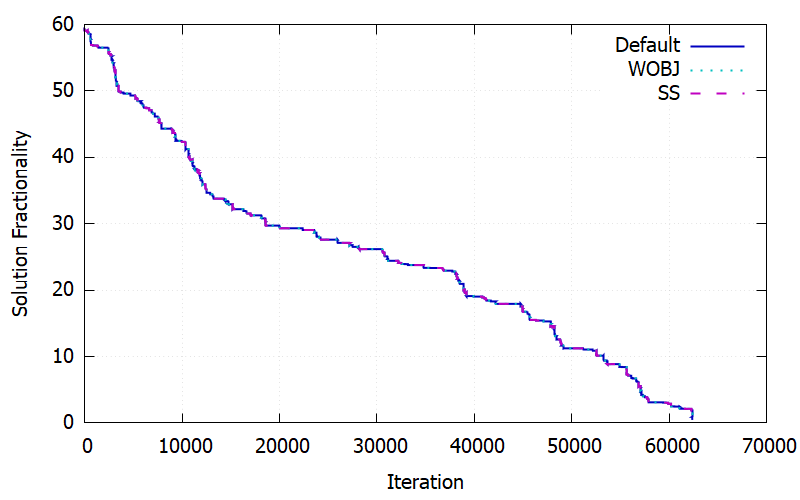
\includegraphics[width=0.85\textwidth]{fast0507-solfrac-worst.png}
	\caption{Solution fractionality of ZI-Round executions for the instance \texttt{fast0507}: worst-performing versions, in terms of number of iterations taken to round all the fractional integer variables.}
	\label{fig:fast0507-solfrac-worst}
\end{figure}

\begin{figure}[h!]
	\centering
	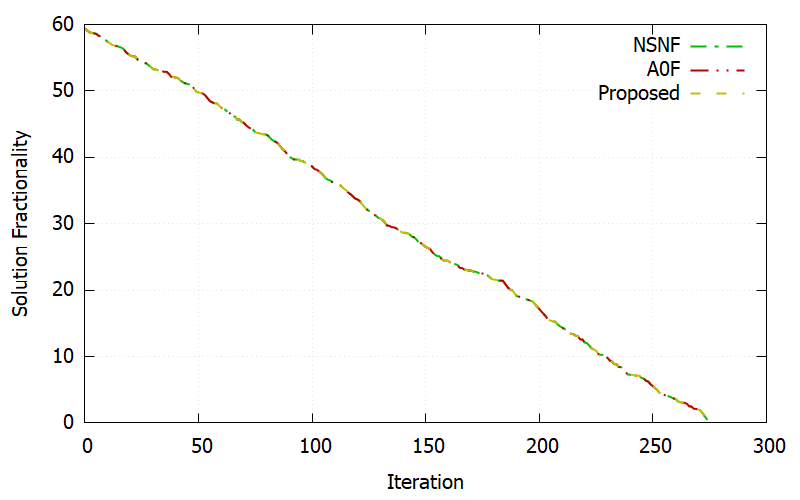
\includegraphics[width=0.85\textwidth]{fast0507-solfrac-best.png}
	\caption{Solution fractionality of ZI-Round executions for the instance \texttt{fast0507}: best-performing versions, in terms of number of iterations taken to round all the fractional integer variables.}
	\label{fig:fast0507-solfrac-best}
\end{figure}

All the three worst-performing versions present the two interfering phases of rounding and objective improvement, whereas all the three best-performing versions present a clear separation of the two phases, or the lack of one. The proposed version of ZI-Round clearly inherits the fast rounding phase from the extension that avoids improving the objective value while roundable fractional integer variables are still available. Notice the high delay in the rounding phase caused by the interference of the objective improvement phase for the instance \texttt{fast0507}: from $275$ iterations in Figure~\ref{fig:fast0507-solfrac-best} to more than $60000$ iterations in Figure~\ref{fig:fast0507-solfrac-worst}. \par
 
%! Solution fractionality seymour
For the instance \texttt{seymour}, the solution fractionality curves of all the ZI-Round versions tested are presented in a single chart in Figure~\ref{fig:seymour-solfrac-all}.

\begin{figure}[ht]
	\centering
	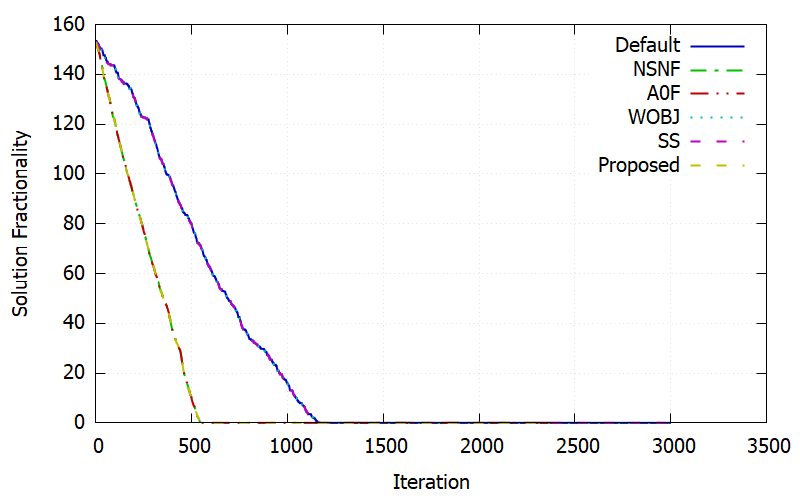
\includegraphics[width=0.85\textwidth]{seymour-solfrac-all.png}
	\caption{Solution fractionality of ZI-Round executions for the instance \texttt{seymour}: all versions.}
	\label{fig:seymour-solfrac-all}
\end{figure}

The same distinction of the worst-performing and best-performing versions made for the instance \texttt{fast0507} applies. In this case, though, the delay in the rounding phase caused by the interference of the objective improvement phase is less significative but still not negligible. As stated before, the proposed version of ZI-Round inherits the fast rounding phase from the extension that avoids improving the objective value while roundable fractional integer variables are still available. \par

%! Solution cost fast0507
For the instance \texttt{fast0507}, the solution cost curves of all the ZI-Round versions tested are presented in a single chart in Figure~\ref{fig:fast0507-solcost-all}. The chart corresponding to the version that does not improve the objective value is also presented as a standalone chart in Figure~\ref{fig:fast0507-solcost-nsnf}, since it is not visible in the main chart, due to its high scale difference with respect to the charts of all the other versions.

\begin{figure}[ht]
	\centering
	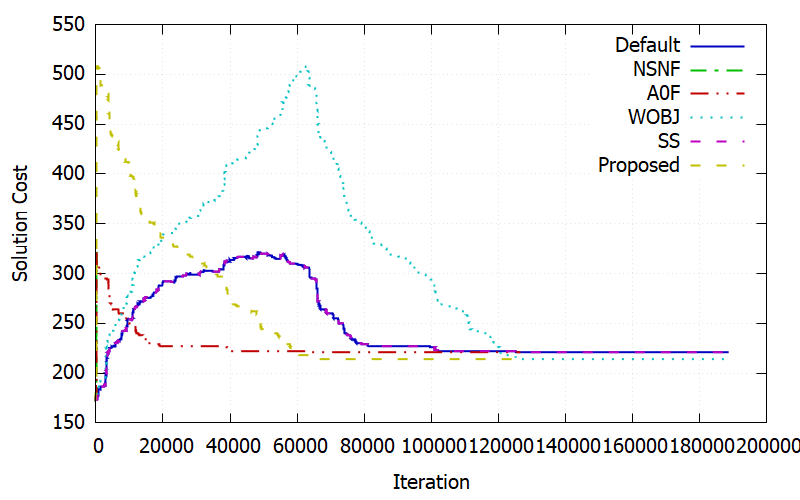
\includegraphics[width=0.85\textwidth]{fast0507-solcost-all.png}
	\caption{Solution cost of ZI-Round executions for the instance \texttt{fast0507}: all versions.}
	\label{fig:fast0507-solcost-all}
\end{figure}

\begin{figure}[h!]
	\centering
	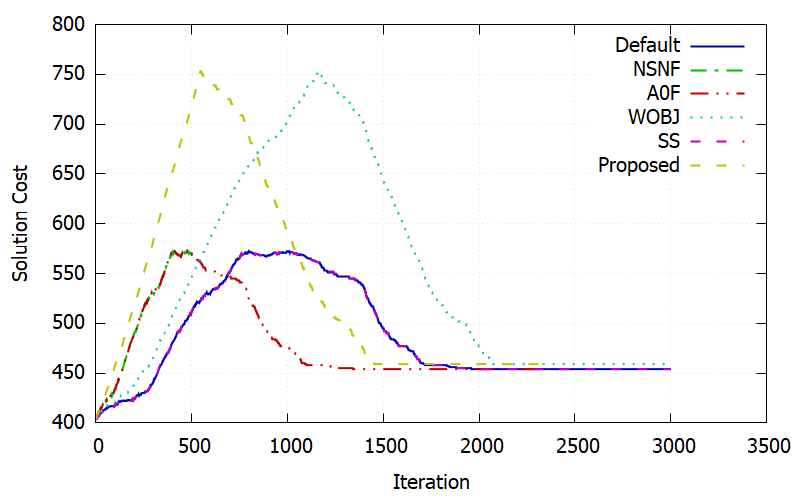
\includegraphics[width=0.85\textwidth]{seymour-solcost-all.png}
	\caption{Solution cost of ZI-Round executions for the instance \texttt{seymour}: all versions.}
	\label{fig:seymour-solcost-all}
\end{figure}

The three versions in which the two phases interfere with one another present a slow worsening of the objective value as the fractional integer variables are being rounded. When the solution fractionality finally reaches zero after more than $60000$ iterations, the objective improvement phase operates alone. 
The effect of rounding variables in the direction that worsens the objective value when fractionality tie-breaks occur is clearly visible in the solution cost curve of the corresponding version.
The two versions in which the two phases are separated, instead, present a fast worsening of the objective value, in terms of number of iterations. As soon as the fast rounding phase ends, the solution cost starts being improved. \par

%! Solution cost seymour
For the instance \texttt{seymour}, the solution cost curves of all the ZI-Round versions tested are presented in a single chart in Figure~\ref{fig:seymour-solcost-all}. The chart corresponding to the version that does not improve the objective value is also presented as a standalone chart in Figure~\ref{fig:seymour-solcost-nsnf}, since it is not visible in the main chart, due to its high scale difference with respect to the charts of all the other versions.

\begin{figure}[ht]
	\centering
	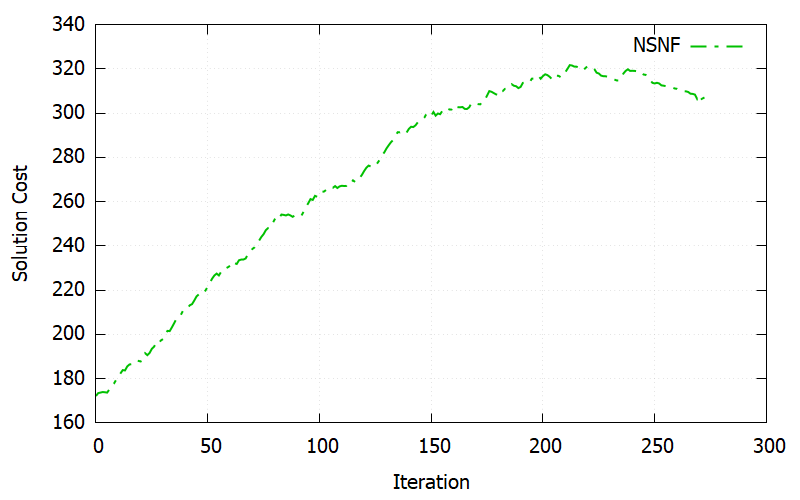
\includegraphics[width=0.83\textwidth]{fast0507-solcost-nsnf.png}
	\caption{Solution cost of ZI-Round execution for the instance \texttt{fast0507}: no objective improvement.}
	\label{fig:fast0507-solcost-nsnf}
\end{figure}

\begin{figure}[h!]
	\centering
	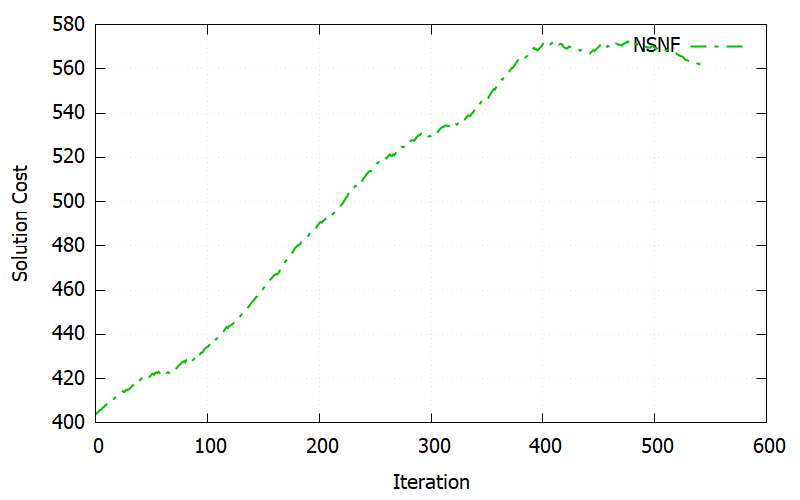
\includegraphics[width=0.83\textwidth]{seymour-solcost-nsnf.png}
	\caption{Solution cost of ZI-Round executions for the instance \texttt{seymour}: no objective improvement.}
	\label{fig:seymour-solcost-nsnf}
\end{figure}

The three versions in which the two phases interfere with one another present the same behavior observed for the instance \texttt{fast0507}, as well as the two versions in which the two phases are separated. \par 

The results obtained and the observations made allow to conclude that the proposed version of ZI-Round inherits its behaviors from the extension that penalizes the objective value when fractionality tie-breaks occur and the extension that keeps the two phases separated, specifically: the magnitude of the objective worsening from the former extension; the faster objective worsening from both extensions; the faster rounding phase from the latter extension.

%\begin{figure}[ht]
%	\centering
%	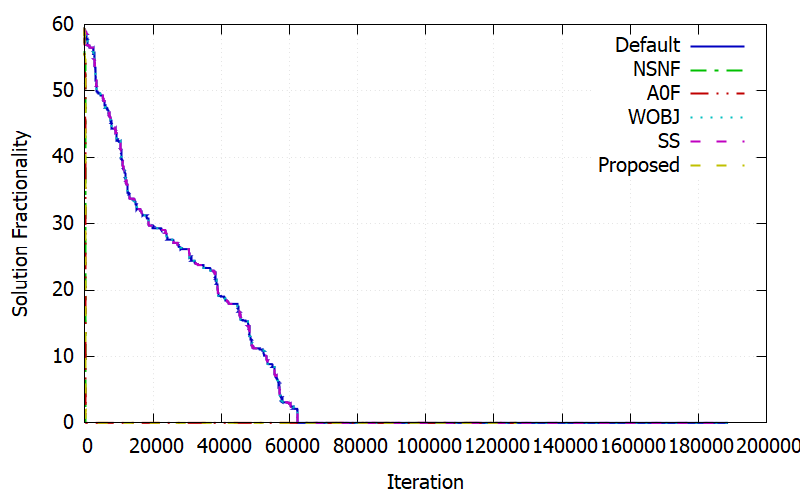
\includegraphics[width=0.85\textwidth]{fast0507-solfrac-all.png}
%	\caption{Solution fractionality of ZI-Round executions for the %instance \texttt{fast0507}: all versions.}
%	\label{fig:fast0507-solfrac-all}
%\end{figure}

%\begin{figure}[ht]
%	\centering
%	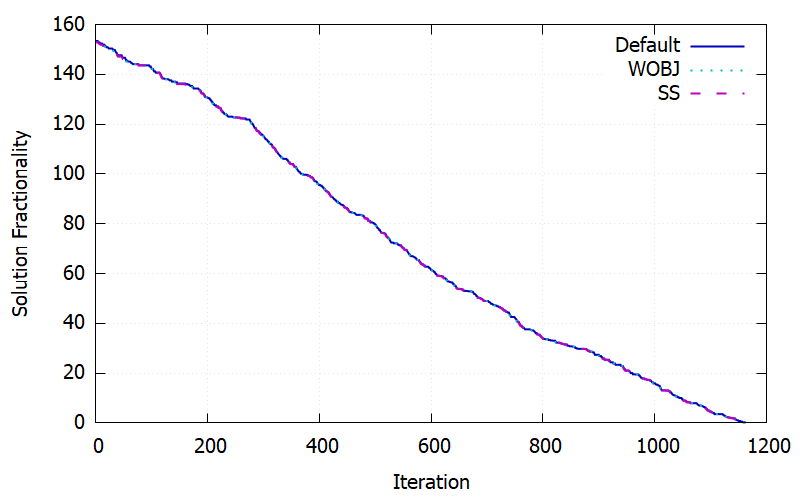
\includegraphics[width=0.85\textwidth]{seymour-solfrac-worst.png}
%	\caption{Solution fractionality of ZI-Round executions for the %instance \texttt{seymour}: worst versions.}
%	\label{fig:seymour-solfrac-worst}
%\end{figure}

%\begin{figure}[ht]
%	\centering
%	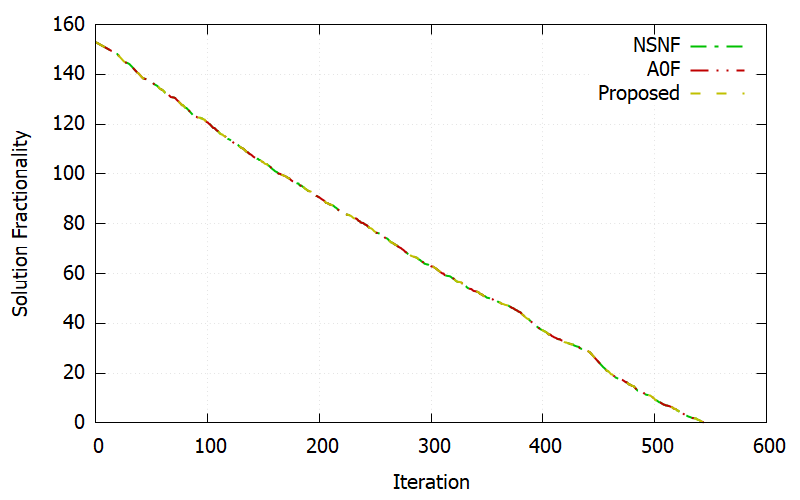
\includegraphics[width=0.85\textwidth]{seymour-solfrac-best.png}
%	\caption{Solution fractionality of ZI-Round executions for the %instance \texttt{seymour}: best versions.}
%	\label{fig:seymour-solfrac-best}
%\end{figure}